\documentclass[10pt,letterpaper,notitlepage]{article}
\usepackage{graphicx}
\usepackage[margin=1in]{geometry}
\usepackage{hyperref}
\hypersetup{colorlinks=true}
\usepackage{amssymb,amsfonts,amsmath,upgreek}
\renewcommand{\familydefault}{\sfdefault}
\usepackage{listings}
\usepackage{courier}
 \lstset{
         basicstyle=\footnotesize\ttfamily, % Standardschrift
         numberstyle=\tiny,          % Stil der Zeilennummern
         numbersep=5pt,              % Abstand der Nummern zum Text
         tabsize=2,                  % Groesse von Tabs
         extendedchars=true,         %
         breaklines=true,            % Zeilen werden Umgebrochen
         keywordstyle=\color{red},
    		frame=b,         
         stringstyle=\color{white}\ttfamily, % Farbe der String
         showspaces=false,           % Leerzeichen anzeigen ?
         showtabs=false,             % Tabs anzeigen ?
         xleftmargin=17pt,
         framexleftmargin=17pt,
         framexrightmargin=5pt,
         framexbottommargin=4pt,
         showstringspaces=false      % Leerzeichen in Strings anzeigen ?        
 }
\setlength{\parskip}{\baselineskip}%
\usepackage{caption}
\usepackage{bm}
\DeclareCaptionFont{white}{\color{white}}
\DeclareCaptionFormat{listing}{\colorbox[cmyk]{0.43, 0.35, 0.35,0.01}{\parbox{\textwidth}{\hspace{15pt}#1#2#3}}}
\captionsetup[lstlisting]{labelformat=empty,format=listing,labelfont=white,textfont=white, singlelinecheck=false, margin=0pt, font={bf,footnotesize}}
%opening
\parindent=0mm


\begin{document}
\title{GROMACS-LS: Computing the Local Stress\\Tensor from MD Simulations}
\author{Juan M.~Vanegas and Alejandro Torres-S\'anchez
\\juan.m.vanegas@gmail.com
\\torres.sanchez.a@gmail.com
\\Universitat Polit\`ecnica de Catalunya-BarcelonaTech, \\Barcelona, Spain.}
\maketitle

\section{Introduction}
This is a manual for GROMACS-LS, a custom GROMACS version to compute the local stress tensor in 3D from a molecular dynamics simulation. This program computes the local stress based on the Hardy stress definition (see Ch.8 in Tadmor \& Miller (2011) {\bf Modeling Materials: Continuum, Atomistic and Multiscale Techniques}). The atomic virial stress (A. P. Thompson et al., J. Chem. Phys. 131, 154107 (2009)) definition was also recently added. Methodological details of the implementation can be found in:

{\bf Importance of Force Decomposition for Local Stress Calculations in Biomembrane Molecular Simulations} by J. M. Vanegas, A. Torres-Sanchez, and M. Arroyo. J. Chem. Theor. Comput.  10, 691 (2014). 

{\bf Examining the Mechanical Equilibrium of Microscopic Stresses in Molecular Simulations} by  A. Torres-S\'anchez, J. M. Vanegas, and M. Arroyo. PRL (2015, in press).

We have patched the GROMACS source code (v4.5.5) at various locations in the routines that calculate particles forces and velocities. Our patches rely heavily on the code structure and functions implemented in a previous local pressure code (obtained from \url{http://repo.or.cz/w/gromacs.git/shortlog/refs/heads/release-4-5-localpressure} and \url{ftp://ftp.gromacs.org/pub/tmp/gromacs-4.0.2_localpressure.tar.gz}). This previous code implements the methodology outlined in

{\bf 3D Pressure Field in Lipid Membranes and Membrane-Protein Complexes} by S. Ollila et al. Phys. Rev. Lett. 102, 078101 (2009). 

\subsection{Highlights of GROMACS-LS}
\begin{itemize}
    \item Decomposition of multi-body potential forces using:
    \begin{enumerate}
	\item Covariant central force decomposition (cCFD) (Torres-S\'anchez A. Vanegas, J. M. and Arroyo, M. (Phys. Rev. Lett., 2015)).
    \item Non-covariant central force decomposition (nCFD) (N. C. Admal and E. B. Tadmor; J. Elast. 100, 63-143, 2010).
    \item Goetz-Lipowsky decomposition (GLD) (R. Goetz and R. J. Lipowsky; J. Chem. Phys. 108, 7397-7409, 1998.). 
    \item Method of planes (Heinz, A.  Paul W. and Binder K. Phys. Rev. E. 72 066704 (2005)).
    \end{enumerate}
	\item Ability to output the total or individual contributions to the local stress such as those from vdw, electrostatics, angles, and others.
	\item Finite discretization over a rectangular grid using tri-linear weight functions, which result in smoother stress fields and also make the discretization exact regardless of the grid size.
	\item Consistent treatment of forces arising from bond constraints (LINCS, SETTLE and SHAKE algorithms), which produces constant profiles for the normal component (perpendicular to the membrane plane) of the stress. This is necessary from an equilibrium stand-point and was an unresolved problem for stress profiles obtained from atomistic membrane simulations.
	\item Virial stress per atom as defined in A. P. Thompson et al., J. Chem. Phys. 131, 154107 (2009). 
\end{itemize}

If you publish results using GROMACS-LS, we kindly ask you to cite the papers by Vanegas et al., Torres-S\'anchez et al., and Ollila et al., which we recommend you to read before continuing with the rest of the manual. In these papers we show the main differences between the different definitions of the stress. We show that the virial stress per atom and the stress from the method of planes do not satisfy balance of linear momentum, while the stress from cCFD, nCFD and GLD do. We also show that the GLD and the stress from the decomposition on geometric centers lead to non-symmetric stresses, which therefore do not satisfy balance of angular momentum. The two flavors of the CFD do satisfy both balance of linear and angular momentum by construction. However, for potentials beyond 4-body, such as CMAP, the nCFD leads to unphysical stresses. We therefore suggest that the cCFD definition is preferred in any case.

The types of interaction potentials that are included in stress calculations and have been tested are the following:

\begin{itemize}
	\item Bonds
	\item Angles
	\item Dihedrals (proper, improper, and Ryckaert-Bellemans)
	\item Constraints (SETTLE and LINCS, SHAKE is included but has not been tested)
	\item Van der Waals
	\item Coulomb (plain cut-off and reaction-field) 
	\item CMAP
\end{itemize}

As such, if you use this code to analyze a system that may use other types of potentials, we cannot guarantee that it will be correct. Please thoroughly check the output of the program and compare to known quantities such as the total pressure. For such comparisons you should first obtain the total virial pressure in double precision. To do this, reanalyze the trajectory (i.e. \texttt{mdrun\_d -rerun}) using a double precision version of GROMACS and recompute the pressure with \texttt{g\_energy\_d}. 

\subsection{Summary of Recent Changes}

The latest version of the code has undergone some significant changes that may affect its usage compared to previous versions:

\begin{itemize}
	\item The code now requires an external LAPACK library. This is need to decompose the higher order potentials such as CMAP, and it also makes the force decomposition much more robust.
	\item In order to be more consistent with the naming and avoid confusion, we have changed all references from pressure to stress. This affects the naming of programs
	
	\texttt{mdrun\_LP} is now \texttt{mdrun\_LS}
	
	and input flags
	
	\texttt{-lpgridx} is now \texttt{-lsgridx}
	
	\item With the addition of new force decompositions the \texttt{-lsfd} has new options: \texttt{ccfd} (covariant central force decomposition, default), \texttt{ncfd} (non-covariant central force decomposition), \texttt{gld} (Goetz-Lipowsky decomposition), or \texttt{mop} (method of planes). We recommend to use \texttt{ccfd}.
	\item A new flag (\texttt{-lssa}) has been added to select whether to calculate the spatial IKN stress as before (option \texttt{spat}, default) or the virial stress per atom (option \texttt{atom})
	\item The CMAP 5-body potential (used in combination with the CHARMM force-field) is now included in the decomposed potentials.
	\item We now include a utility called \texttt{tensortools} which replaces the individual c utilities \texttt{bin2xvg}, \texttt{bin2ncdf}, etc.
\end{itemize}

\section{Installation}
GROMACS-LS is based on GROMACS version 4.5.5. While the vanilla 4.5.5 version can be compiled using both the autoconf tools and CMake, this custom GROMACS-LS version can only be compiled with CMake.

External requirements: FFTW3, LAPACK

You will need to install a recent version of the FFTW3 library (in double precision and as shared library), CMake, and LAPACK (http://www.netlib.org/lapack). The LAPACK library needs to be installed as a shared library (.so). Compiling LAPACK with the autoconf tools can be hassle, but recent versions can be easily compiled and installed with CMake.

\begin{lstlisting}[caption=Installing LAPACK with CMake]
$> tar -zxvf lapack-3.5.0.tgz
$> cd lapack-3.5.0
$> mkdir build
$> cd build
$> ccmake ../
\end{lstlisting}

Once the \texttt{ccmake} dialog comes up, press c to begin the initial configuration. Change the \texttt{BUILD\_SHARED\_LIBS} flag to ON and modify the \texttt{CMAKE\_INSTALL\_PREFIX} variable to set the target installation directory. After ccmake quits, you can follow the standard linux installation commands of \texttt{make} and \texttt{make install}.

If you install FFTW3 and LAPACK with a linux distribution such as Ubuntu or Fedora, you will also need to install the development (header) packages. If you have installed the FFTW3 or LAPACK libraries in a non-standard location (i.e. other than /usr/lib or /usr/local/lib), then before running \texttt{ccmake} you should export the variables \texttt{FFTW3\_ROOT\_DIR} and \texttt{CMAKE\_PREFIX\_PATH}, e.g.

\texttt{export FFTW3\_ROOT\_DIR=/path/to/fftw3}

\texttt{export CMAKE\_PREFIX\_PATH=/path/to/lapack}

Now the installation of the custom GROMACS-LS package

\begin{lstlisting}[caption=Installing LAPACK with CMake]
$> tar -zxvf gromacs-4.5.5-ls-5.0.tar.gz
$> cd gromacs-4.5.5-ls-5.0
$> mkdir build
$> cd build
$> ccmake ../
\end{lstlisting}

Once the \texttt{ccmake} dialog comes up, press c to begin the initial configuration, and then modify the \texttt{CMAKE\_INSTALL\_PREFIX} variable to set the target installation directory. Use the toggle feature of \texttt{ccmake} (press t) and check that the paths to the FFTW3 and LAPACK libraries are correct.

Do not modify other variables unless you KNOW what you are doing. By default, the code is compiled in double precision (this is absolutely necessary), it cannot be compiled with MPI or GPU support, and all programs have the suffix \_LS. Press c again and then g to generate the necessary Makefiles.

After ccmake quits, you can follow the standard linux installation commands of \texttt{make} and \texttt{make install}.

In addition to the GROMACS-LS code, we have also included two python programs:

\texttt{LStensor.py} and \texttt{tensortools}

\texttt{LStensor.py} contains a number of modules that can be imported into other python programs for the analysis of the data produced with the GROMACS-LS software. The \texttt{tensortools} utility provides an easy to use command line interface to most of the modules available in the \texttt{LStensor.py} file. These two files are installed along with the other GROMACS-LS files in the bin folder. We discuss these tools in more detail in Section \ref{postprocess}.

\section{Using the Code}

\subsection{Analyzing an MD Trajectory}

For calculating the stress tensor in a MD simulation, we need a trajectory file (\texttt{.trr}) that contains both positions and velocities at the same points in time. In this section we show the steps you need to follow to calculate the stress tensor and illustrate it in the particular case of a POPE membrane. 

As individual components of the system may drift over time, e.g. a membrane may drift in the simulation box, it is a good idea to first center a given group of atoms (in this case, the POPE bilayer) in the center of the simulation box. To do so, we use the tool \texttt{trjconv\_LS} with the original trajectory, \texttt{traj.trr}:
\begin{lstlisting}[caption=Center the molecule into the simulation box before analyzing the stress]
$ trjconv_LS -f traj.trr -o traj_centered.trr -n index -center -s topol.tpr

(...)

Select group for centering
Group     0 (         System) has 11600 elements
Group     1 (           POPE) has  2600 elements
Group     2 (          Water) has  9000 elements
Select a group: 1
\end{lstlisting}
Note that this \texttt{trjconv\_LS} is a modified version of the vanilla one that places the center of mass, and not the geometrical center as it is done by the original, of the selected index group at the center of the simulation box. You must always pass a \texttt{.tpr} file as part of the input, or the program will return a segmentation fault without an error message. This new \texttt{traj\_centered.trr} is the trajectory we will use to analyze the stress.

The 3D stress tensor is obtained by ``rerunning'' the trajectory with the \texttt{mdrun\_LS}. Since the \texttt{-rerun} option of \texttt{mdrun\_LS} outputs new \texttt{.log}, \texttt{.edr}, and \texttt{.trr} files, we suggest you first create a new folder and analyze the trajectory within it:
\begin{lstlisting}[caption=Computing the stress with \texttt{mdrun\_LS}]
$ mkdir stress
$ cd stress
$ mdrun_LS -s ../topol.tpr -rerun ../traj_centered.trr
\end{lstlisting}
To save space you can recreate the \texttt{.tpr} file by setting all the output \texttt{nst*} variables to 0 in the \texttt{.mdp} file:

\texttt{nstxout         = 0\\
nstvout         = 0\\
nstlog          = 0\\
nstenergy       = 0\\
nstxtcout       = 0\\
}

If your simulation was performed with PME or another long-range electrostatic method, you will need to create a new \texttt{.tpr} file with the \texttt{coulombtype} set to \texttt{Cut-off} or \texttt{Reaction-field} and a cutoff radius of at least 2.0-2.2 nm (see the Ref. 2 for more details). Note that this does not change your original trajectory but the way forces are calculated when analyzing each frame.

As with other Gromacs tools, \texttt{mdrun\_LS} displays a help text running \texttt{mdrun\_LS -h}. \texttt{mdrun\_LS} has several special options for analyzing the stress:
\begin{lstlisting}[caption=\texttt{mdrun\_LS} special options]
Option     Filename  Type         Description
------------------------------------------------------------
-ols localstress.dat  Output       Generic data file

Option       Type   Value   Description
------------------------------------------------------
-localsgrid  real   0.1     Spacing for local pressure grid (default = 0.1 nm)
-lsgridx     int    0       Set the local pressure grid size in the x
                            direction (default use box[XX][XX]/localsgrid)
-lsgridy     int    0       Set the local pressure grid size in the y
                            direction (default use box[YY][YY]/localsgrid)
-lsgridz     int    0       Set the local pressure grid size in the z
                            direction (default use box[ZZ][ZZ]/localsgrid)
-lscont      string all     Select which contribution to write to output
                            (default = all): all, vdw, coul, angles, bonds,
                            dihp, dihi, dihrb, lincs, settle, shake, cmap, vel
-lsfd        string ccfd    Select the type of force decomposition to be
                            used: ccfd (covariant central force
                            decomposition, default), ncfd (non-covariant
                            central force decomposition), gld (Goetz-Lipowsky
                            decomposition), or mop (method of planes)
-lssa        string spat    Select the type of stress to calculate: spat
                            (spatial stress from IKN theory, default), atom
                            (stress per atom)

\end{lstlisting}
With the flag \texttt{-ols} one selects the output file where the stress tensor is stored. The size of the discretization grid is given by several parameters. If your system was simulated at constant pressure, the program takes the size of the box (box[XX], box[YY], box[ZZ]) from the \texttt{.tpr} along with the desired grid spacing (with \texttt{-localsgrid}), and calculates the integer size of the grid and the real grid spacing, e.g. if the box size in the x direction is 5.37 nm and the given grid spacing is 0.1 nm, then the grid size in x is 53 and the real grid spacing becomes 0.1013 nm. The grid size in each dimension can also be overridden with the \texttt{-lsgridx}, \texttt{-lsgridy}, or \texttt{-lsgridz}. So if you are interested in calculating a stress profile along a given dimension, e.g. z, then you can use these different flags together:
\begin{lstlisting}[caption=Setting the grid size]
$ mdrun_LS -s ../topol.tpr -rerun ../traj_centered.trr -localsgrid 0.1 -lsgridx 1 -lsgridy 1
\end{lstlisting}
%check to use simulations with non-rectangular boxes - use trjconv to change
At the moment, only systems simulated with rectangular boxes can be analyzed. \texttt{mdrun\_LS} can also return the total or individual contributions to the stress with the \texttt{-lscont} flag. At the moment the available contributions are van der Waals, Coulomb, angles, bonds, proper dihedrals, improper dihedrals, Ryckaert-Bellemans dihedrals, constraints (LINCS, SHAKE, or SETTLE), cmap, and kinetic. 

Finally, the \texttt{-lsfd} flag allows to select one of two different decompositions for the forces between particles that enter into the potential part of the stress. We advice you to use the ccfd option (set by default in the program) that always provides a symmetric stress, thereby satisfying the balance of angular momentum from a continuum viewpoint, and physically meaningful regardless of the number of particles involved in each additive potential of the force field. The ncfd is equivalent to the ccfd except for 5-body potentials. On the other hand, the gld option allows you to compute the stress from the decomposition by Goetz and Lipowsky (J. Chem. Phys. (1998) 17, 7397-7409), which has been widely used in biomembrane simulations. Please, take a close look to references 2 and 3 for a more detailed discussion about the differences between both decompositions.


The outputted \texttt{.dat0} file is a simple binary file in double precision with the following format:
\begin{lstlisting}[caption=Format of the \texttt{.dat0} binary file]
precission   = sizeof(int)*1
box          = sizeof(double)*9
gridx        = sizeof(int)*1
gridy        = sizeof(int)*1
gridz        = sizeof(int)*1
stresstensor = sizeof(double)*9*gridx*gridy*gridz
\end{lstlisting}

\subsection{\texttt{tensortools}: Python scripts to post-process the stress fields \label{postprocess}}

The command \texttt{mdrun\_LS} produces binary \texttt{.dat0} files that need to be post-processed for analysis. To make life easier, we have included two tools \texttt{tensortools} and \texttt{LStensor.py} that can load, transform and save these binary files in useful formats. These python files are directly installed to the binary folder of the GROMACS\_LS distribution. These python utilities require recent versions of the Numpy and Scipy packages, and optionally the ProDy package (http://prody.csb.pitt.edu/) when using some of the stress per atom options.

\subsubsection{LStensor}
The \texttt{LStensor.py} file defines what we call the LStensor object and corresponding analysis functions, which can be used to post-process the data from the GROMACS\_LS program. This object can load IKN stresses as well as stresses per atom and convert these to a grid. It can also be used to compute the basic invariants of the stress as well as its divergence. It also provides a number of functions to load PDB files (stress per atom only) and to store files in NETCDF, plain txt, and PDB format.

\subsubsection{tensortools}
The other file, \texttt{tensortools}, is a command-line utility that can be used for a rapid post-processing of the binary stress files. It uses the functions defined in \texttt{LStensor.py} and allows easy manipulation of the data. The main options are:

\begin{lstlisting}[caption=Options for tensortools (tensortools -h)]
-h, --help            show this help message and exit
-f [input.bin] [[input.bin] ...]
                      Single or multiple binary input files (must all have
                      the same grid size)
-v []                 verbose
--irep [spat]         Input data representation, values: spat (spatial
                      stress/density distributed on a grid, default), atom
                      (stress per atom)
--pdb [[structure.pdb]]
                      PDB file with atom coordinates (FOR STRESS PER ATOM
                      ONLY)
--itype [stress]      Type of data such as density, stress tensor, or vector
                      field: dens, stress (default), or vec
--mif [avg]           How to process multiple input files, values: avg
                      (default) or sum
--sym []              FOR STRESS ONLY. Separates the resultant stress in its
                      symmetric and antisymmetric parts, and creates two
                      outputs with the subscripts _sym and _asym
                      respectively
--prof z              Output a profile along a given dimension, values: x,
                      y, or z (default)
--integ z             integrate out the stress profile along a given
                      dimension, values: x, y, or z (default)
--gf 1.0              Process input through a gaussian filter of a given
                      standard deviation (in units of the grid spacing, default=1.0)
--gridsp 0.1 0.1 0.1  (For atom to grid conversion) Grid spacing for atom 2
                      grid conversion (default 0.1, 0.1, 0.1 nm)
--orep [spat]         Output data representation, values: spat (spatial
                      stress/density distributed on a grid, default), atom
                      (stress per atom)
--oformat [bin]       Output format, values: bin (i.e. binary .dat0,
                      default), nc (NETCDF), txt (default when using --prof),
                      or pdb (stress per atom only, creates a separate file for
                      each element in the tensor)
-o output.bin         Output file
  
\end{lstlisting}

Some examples of basic usage:

\begin{lstlisting}[caption={Averaging multiple input *.dat0 files}]
tensortools -f file0.dat0 file1.dat0 file2.dat0 -o stress.dat0
\end{lstlisting}

\begin{lstlisting}[caption={Conversion to NETCDF format}]
tensortools -f file.dat0 --oformat nc -o stress.nc
\end{lstlisting}

\begin{lstlisting}[caption={Compute a stress profile along the y axis and saves it to a text file}]
tensortools -f file.dat0 --prof y -o stress.txt
\end{lstlisting}

\begin{lstlisting}[caption={Smooth data using a gaussian kernel with a standard deviation of 8 (in units of the grid spacing)}]
tensortools -f file.dat0 --gf 8.0 -o stress.dat0
\end{lstlisting}

Advanced usage:

\begin{lstlisting}[caption={Read the IKN stress from *.dat0 files, integrate out the z direction, smooth the data with a Gaussian filter of 25 (units of the grid size), and write the result in the file stress\_gf25.nc}]
tensortools -f *.dat0 --inte z --oformat nc --gf 25 -o stress_gf25.nc -v
\end{lstlisting}

\begin{lstlisting}[caption={Read the stress per atom from *.dat0 files, load the PDB structure from struct.pdb, translate the data to a grid with spacing 0.01, 0.01, 10, apply a Gaussian filter of 25 and store the result in stress\_atom\_gf25.nc}]
tensortools -f *.dat0 --irep atom --pdb struct.pdb  --orep spat --oformat nc -o stress_atom_gf25.nc --gridsp 0.01 0.01 10 --gf 25 -v
\end{lstlisting}

Note that although the main purpose of \texttt{LStensor.py} and \texttt{tensortools} is to analyze the stress tensor binary files, it can also manipulate other binary files such as those outputted by the \texttt{g\_density3D\_LS} utility. 

\section{Some technical comments about cCFD and nCFD}

In the new version of the code, computing any flavor of the central force decomposition (cCFD and nCFD) for a given potential $V_I$ is done by solving the overdetermined system of equations
\begin{equation}
\label{system}
\bm{F}_I^\alpha = \sum_{\beta\in\mathcal{I}_I,\beta\neq\alpha}  \bm{f}^{\alpha\beta}= \sum_{\beta\in\mathcal{I}_I,\beta\neq\alpha}  \varphi^{\alpha\beta}\frac{\bm{r}^{\alpha\beta}}{|\bm{r}^{\alpha\beta}|}, \forall \alpha \in \mathcal{I}_I
\end{equation}
where $\mathcal{I}_I$ is the set of particles interacting through the potential $V_I$, $\bm{f}^{\alpha\beta}$ are the terms of the force decomposition and $\varphi{\alpha\beta}$ are their respective magnitudes. If $n_I$, the number of particles involved in the potential, is equal or smaller than 4, this overdetermined system has a single solution and thus cCFD and nCFD coincide. For potentials beyond 4-body, such as the CMAP interaction, this systems becomes underdetermined with an infinite number of possible solutions. We have recently proposed a preferred CFD based on covariance arguments (Torres-S\'anchez et al., in preparation), which we call cCFD. To compute this cCFD we first need to compute a solution to Eq.~\eqref{system}. We do this by calling the DGELSD function of the LAPACK library (\url{http://www.netlib.org/lapack/explore-html/db/d6a/dgelsd_8f.html}) which solves under- and overdetermined linear systems by computing the solution with minimum norm. The solution to this problem is a CFD, which we call nCFD (non-covariant central force decomposition). To compute the cCFD, nCFD is projected onto the tangent plane to the Shape Space, which is calculated through the derivative of Caley-Menger determinants. While nCFD depends on the parametrization of the potential and give spurious results, we have recently proven that cCFD is independent of the representation of the potential and gives physically relevant results (see Torres-S\'anchez et al., for more details). 

\subsection{Frequently Asked Questions}

\begin{description}

\item[Q1. How long does it take to analyze a trajectory with \texttt{mdrun\_LS}?] This depends on the size of your system and the grid size. Analysis time increases with a larger system and a finer grid. For a typical system with approximately 100,000 atoms and a grid spacing of 0.1 nm it can take 5-10 minutes (depending on your hardware) to analyze each frame in the trajectory. The code does not utilize any of the SIMD or GPU optimizations that the vanilla GROMACS uses and therefore is much slower.

\item[Q2. \texttt{mdrun\_LS} has been stuck on the first frame of the trajectory for hours, what's wrong?] If the analysis is taking an unusually long time there may be something wrong with the input files or there may be an unknown problem with the code. You can check this by selecting to output only one of the components such as kinetic one (using the \texttt{-lscont vel} flag), which should be done very quickly even for a large number of particles. If this fails there may be a problem with the trajectory, otherwise there may a particular problem with some of the interactions being calculated. You can try calculating some of the other individual components in order to narrow it down and contact us regarding a particular issue.

\item[Q3. I get a segmentation fault when running \texttt{mdrun\_LS}] Make sure that \texttt{mdrun\_LS} is run in a different folder than where the input trajectory is at, otherwise the program may inadvertently overwrite the input trajectory and cause the error.

\item[Q4. Can the program be run in parallel? ] Not directly. The program must always be run serially. However, each frame in a trajectory can be analyzed completely independent of every other frame. So one method to parallelize the analysis is to separate the trajectory into smaller chunks with equal number of frames (using \texttt{trjconv\_LS -split}), and analyze each chunk separately. You can then average all of the resulting stress files together using the \texttt{tensortools} utility. The advantage of this method is that it always scales linearly although it takes a bit of work to set up. CAUTION! When doing this make sure to use the same \texttt{.tpr} file and same grid spacing to analyze each chunk of the trajectory, otherwise the grid sizes may differ and the average will fail.

\item[Q5. Are the velocities needed?] Absolutely! The kinetic contribution to the stress cannot be calculate without the velocities, and this is a pretty substantial contribution to the total stress.

\item[Q5. Can I use an \texttt{.xtc} file instead of a \texttt{.trr} file?] No. The \texttt{.xtc} file only stores the positions and not the velocities.

\item[Q6. Does \texttt{mdrun\_LS} use the positions and velocities from the \texttt{.tpr} file?] No, \texttt{mdrun\_LS} only uses the positions and velocities stored in the \texttt{.trr} trajectory. However, the initial box size, and therefore the grid size are determined from the values in the \texttt{.tpr} file.

\item[Q7. Are electrostatic contributions calculated using PME included in the stress tensor?] No. At the moment, electrostatic contributions calculated in reciprocal space are not included in the local stress calculation. If you ran your simulation with PME electrostatics, you must change the \texttt{coulombtype} to \texttt{Cut-off} and select an appropriate cut-off value (\texttt{rcoulomb}) in the \texttt{.mdp} file. Then, you can create a new \texttt{.tpr} with \texttt{grompp\_LS}. We recommend to use an \texttt{rcoulomb} value of at least 2.0 - 2.2 nm. CAUTION! The electrostatic contribution to the stress is one of the most computationally intense due to the large number of pair interactions in a typical simulation. The number of interactions increases cubically with the cut-off radius. In our experience, using a cut-off beyond 3.0 nm is computationally unfeasible for normal systems. See Vanegas et al. (JCTC 2014) for more details.

\item[Q8. What is the relation between stress and pressure?] The pressure tensor, $P_{ij}$, has the opposite sign as the stress tensor, $\sigma_{ij}$, so $P_{ij} = -\sigma_{ij}$

\item[Q9. The total stress obtained with \texttt{GROMACS-LS} does not match the pressures obtained with \texttt{g\_energy}] First, if you simulated your system with PME electrostatics and re-analyze with a Cut-off, then the total stress values will never match the virial pressures calculated by GROMACS unless you use an infinite cut-off. See Vanegas et al. (JCTC 2014) for more details. Also, the values obtained from the single precision \texttt{.edr} file generated during the simulation run are not accurate. To do a meaningful comparison you need to reanalyze the trajectory (i.e. \texttt{mdrun\_d -rerun}) using a double precision version of GROMACS and recompute the pressure with \texttt{g\_energy\_d}.

\item[Q10. Is it normal for the local stress values to be so large?] The local stress can easily reach values up to several thousand bars depending on the system and types of interactions.

\begin{figure}[!ht]
\centering
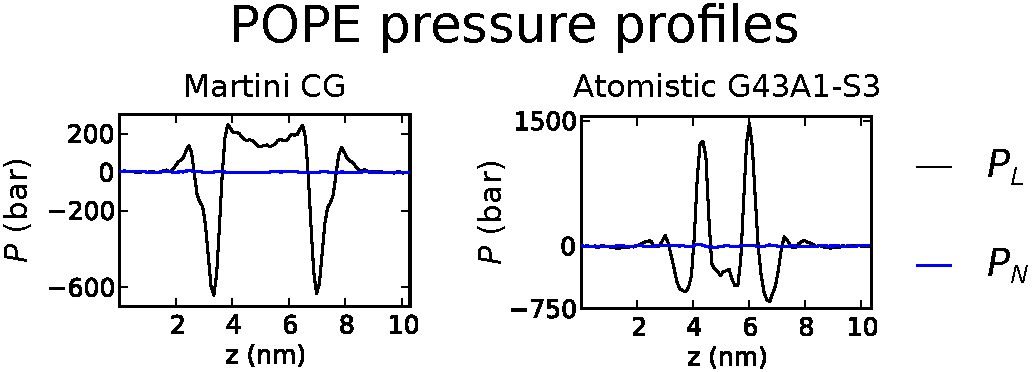
\includegraphics[width=5.5in]{figs/tot.pdf}
\caption{Comparison of stress profiles ($P_N = -\sigma_{zz}$ and $P_L = -(\sigma_{xx} + \sigma_{yy})/2$) for bilayer systems simulated with coarse grained and atomistic force-fields.}
\end{figure}

\item[Q11. How often should I save frames to the trajectory? How long does the simulation need to be?] The answer to this may differ depending on the system. For lipid bilayer systems we typically save frames to the trajectory every 5 or 10 ps, and analyze a 100 ns trajectory. The following shows the improvement in the convergence of the stress profile depending on the number of frames used:

 \begin{figure}[!ht]
 \centering
 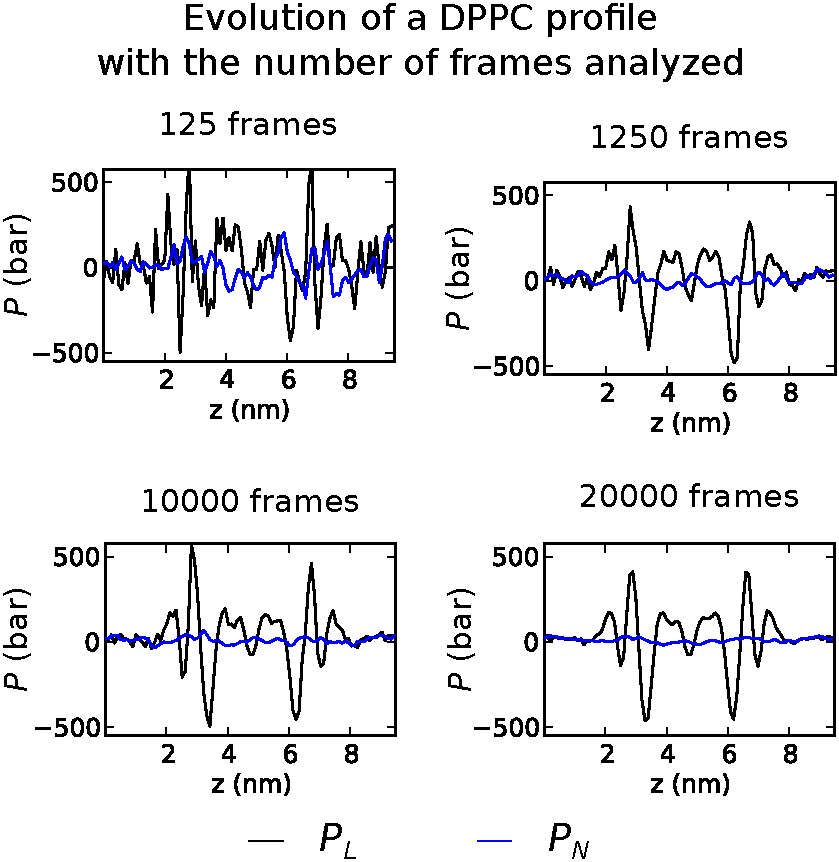
\includegraphics[width=4in]{figs/evol.pdf}
 \caption{}
 \end{figure}

\item[Q12. Why is the normal component (e.g.~$\sigma_{N}$) of the stress profile of my bilayer system not zero?] Mechanical equilibrium dictates that the component of the stress along the direction normal to a lipid bilayer should be constant. The average value of this constant component should match the imposed value of the simulation pressure for the given dimension, which may or may not be zero. The important point is that it should be constant. If $\sigma_{N}$ is not constant (beyond reasonable noise) then there could be several problems with the simulation. First, check that the lipid membrane is fully equilibrated. In our systems composed of 200 lipids (100 lipids in each leaflet) in the liquid phase we equlibrate for 400 ns before running the data collection period. Second, check the \texttt{comm\_grps} option in the \texttt{.mdp} file. Bilayer systems are often simulated with center of mass motion removal done on different groups separately, e.g. \texttt{comm\_grps = BILAYER SOL}. However, doing this will change the internal mechanical behavior of the system. For local stress analysis this \texttt{grompp} option should always be set \texttt{comm\_grps = System} during the simulation run.

\item[Q13. Can the 3D stress tensor be loaded into other programs for visualization?] Yes. The easiest way to do this is to first convert the binary stress file to the NETCDF format using the \texttt{tensortools} utility. You can then load this generic NETCDF file into programs such as UCSF Chimera or Paraview.

\begin{figure}[!h]
\centering
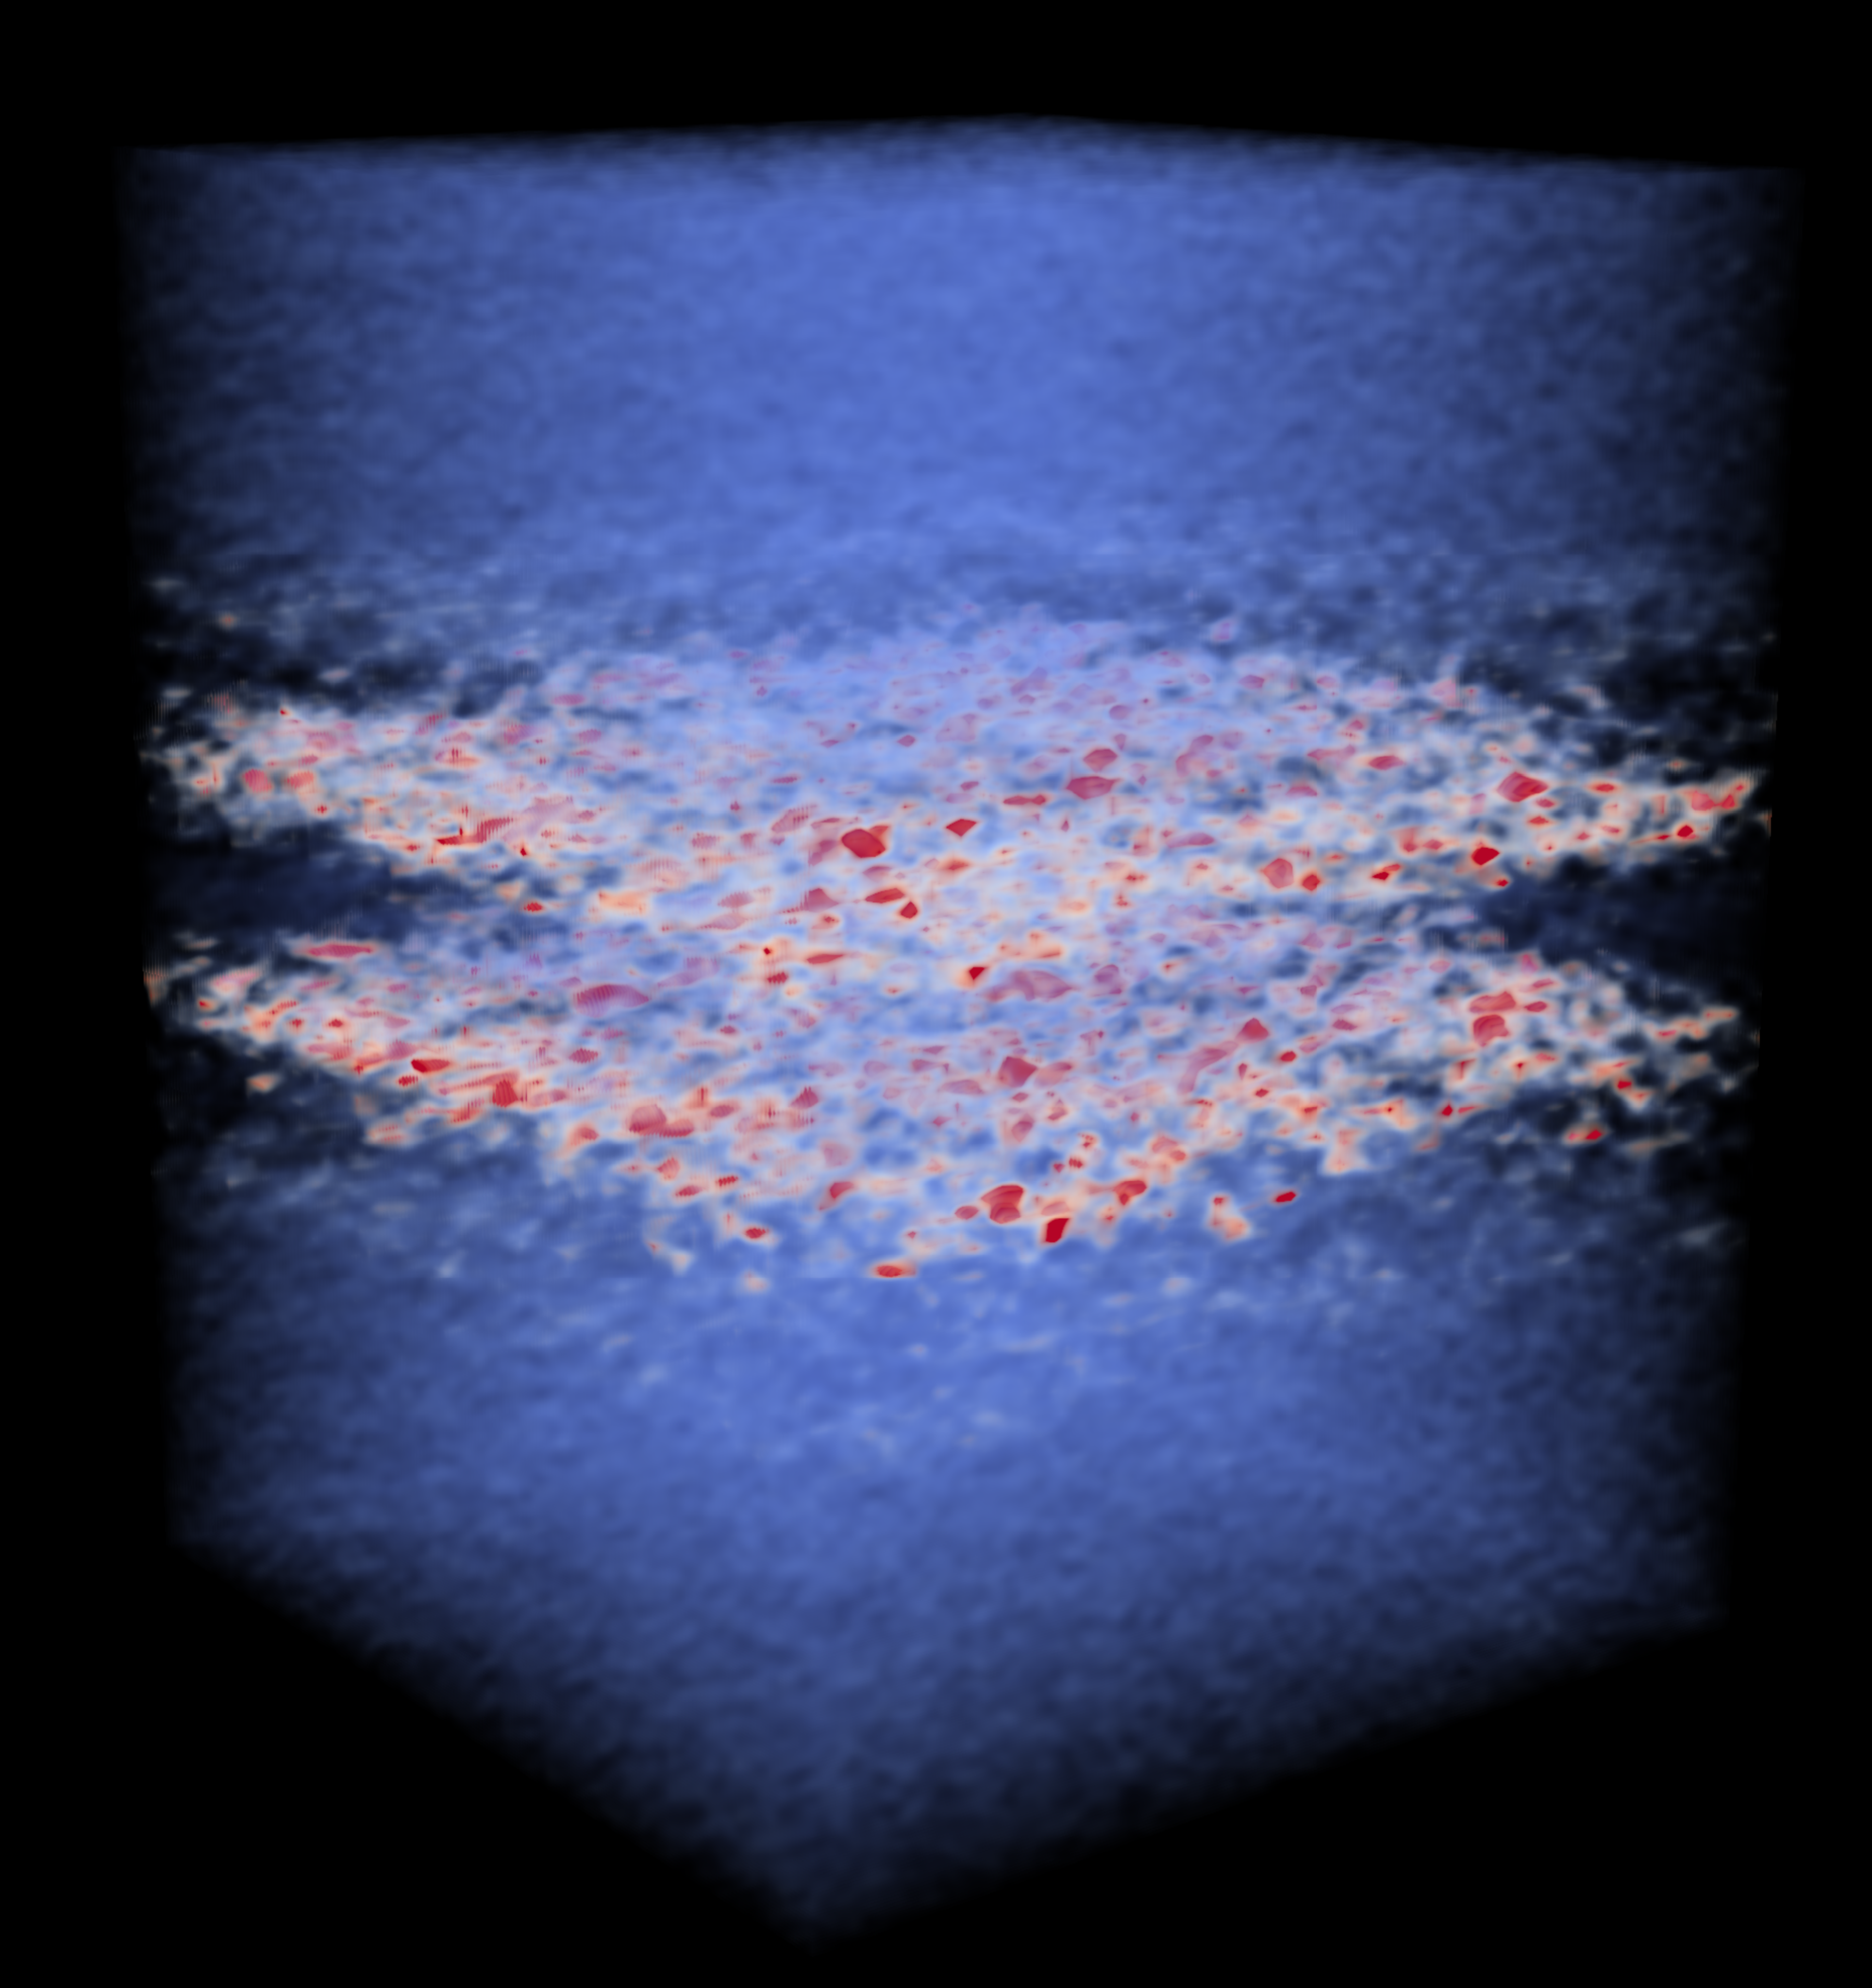
\includegraphics[width=4in]{figs/3D_stress_black_bw.pdf}
\caption{3D stress tensor for a bilayer system visualized in Paraview}
\end{figure}

\end{description}


\end{document}
